\documentclass[conference]{IEEEtran}
%% INFOCOM 2014 addition:
\makeatletter
\def\ps@headings{%
\def\@oddhead{\mbox{}\scriptsize\rightmark \hfil \thepage}%
\def\@evenhead{\scriptsize\thepage \hfil \leftmark\mbox{}}%
\def\@oddfoot{}%
\def\@evenfoot{}}
\makeatother
\pagestyle{headings}

\usepackage{url}
\usepackage{graphicx}
\usepackage{subfigure}
\usepackage{color}

\newcommand{\noteperso}[1]{\begin{center}
\fbox{\begin{minipage}{0.9\columnwidth}#1\end{minipage}}\end{center}}
%\renewcommand{\noteperso}[1]{}

\begin{document}

\title{Measuring the Degree Distribution of Routers\\ in the Core Internet}

\author{
\IEEEauthorblockN{Matthieu Latapy}
\IEEEauthorblockA{LIP6 -- CNRS and UPMC\\ \url{Matthieu.Latapy@lip6.fr}}
\and
\IEEEauthorblockN{\'Elie Rotenberg}
\IEEEauthorblockA{LIP6 -- ENS de Lyon, UPMC\\ \url{Elie.Rotenberg@lip6.fr}}
\and
\IEEEauthorblockN{Christophe Crespelle}
\IEEEauthorblockA{LIP -- Lyon 1 and CNRS\\ \url{Christophe.Crespelle@inria.fr}}
\and
\IEEEauthorblockN{Fabien Tarissan}
\IEEEauthorblockA{LIP6 -- CNRS and UPMC\\ \url{Fabien.Tarissan@lip6.fr}}
}

\maketitle

\begin{abstract}
Most current models of the internet rely on knowledge of the degree distribution of its core routers, which plays a key role for simulation purposes. In practice, this distribution is usually observed directly on maps known to be partial, biased and erroneous. This raises serious concerns on the true knowledge one may have of this key property. Here, we design an original measurement approach targeting reliable estimation of the degree distribution of core routers, without resorting to any map. It consists in sampling random core routers and precisely estimate their degree thanks to probes sent from many distributed monitors. We run and assess a large-scale measurement following this approach, carefully controlling and correcting bias and errors encountered in practice. The estimate we obtain is much more reliable than previous knowledge. It gives evidence of the fact that the degree distribution certainly is not a power-law, in contrast with claims from previous measurements.
\end{abstract}

%\noteperso{si trop long : rapetisser les figures de graphes, mettre la table 2 sur 2 colonnes, virer une ou deux refs (OSN), ...}

%\noteperso{page web outils+data}

%%%%%%%%%%%%%%%%%%%%%%%%%%%%%%%%%%%%%%%%%%%%%%%%%%%%%%%%%%%%%%%%%%%%
%%%%%%%%%%%%%%%%%%%%%%%%%%%%%%%%%%%%%%%%%%%%%%%%%%%%%%%%%%%%%%%%%%%%
\section{Introduction} \label{sec:intro}
%%%%%%%%%%%%%%%%%%%%%%%%%%%%%%%%%%%%%%%%%%%%%%%%%%%%%%%%%%%%%%%%%%%%
%%%%%%%%%%%%%%%%%%%%%%%%%%%%%%%%%%%%%%%%%%%%%%%%%%%%%%%%%%%%%%%%%%%%

The internet has become a crucial infrastructure sustaining our social, economic, cultural and scientific lives at both local and worldwide scales. Despite this, due to its history, its decentralized nature and its mere complexity, our understanding of its global structure remains very limited. In particular, it is now clear that precise knowledge of its components (devices, connections, protocols, etc) is not sufficient to understand its global structure. As a consequence, much effort is nowadays devoted to measurements of the internet, aimed at shedding light on these features~\cite{caida,dimes,iplane,planetlab,ripeatlas}.

One of the main approaches consists in modeling the internet as a graph where nodes are ASes, routers, end-hosts, and/or other devices, and links are physical connections, AS peering, IP neighborhood, etc. One then conducts measurements based typically on traceroute, BGP and/or anti-aliasing in order to build maps of the internet \cite{dimes,routeviews,ripe-ris,caida}. These maps are {\em partial} views of the corresponding graphs, and the underlying object is not always clearly defined \cite{roughan201110}. In addition, such maps may be {\em biased} by the measurement procedure \cite{willinger,DBLP:conf/infocom/LakhinaBCX03,DBLP:journals/jacm/AchlioptasCKM09,DBLP:journals/tcs/DallAstaABVV06,DBLP:journals/cn/GuillaumeLM06,DBLP:conf/infocom/LatapyM08}.  They contain indeed much {\em erroneous} data, due for instance to silent routers, dynamic routing (load balancing in particular), incorrect anti-aliasing \cite{alias-bias,keys2010internet,paristraceroute}. This means that the properties of obtained maps may differ very significantly from the properties of the true graph, in a way that is extremely difficult to assess and correct.

We explore here a completely new approach, based on the idea that one does not need a map to estimate a given property of interest. Instead, we propose to design and perform a measurement procedure targeting the estimation of a specific property. The challenge is then to ensure that the measurement succeeds in giving a reliable estimate.

We focus on the degree distribution of core routers, {\em i.e.} the fraction of core routers with $k$ links for any $k$. The links we consider here are the {\em physical links} of the router, identified by its IP interfaces. We design a measurement procedure able to reliably estimate this distribution. We then develop tools needed to run it, and perform a large-scale measurement from hundreds of monitors distributed in the internet. We obtain this way an estimate of the degree distribution of routers that is much more reliable than previous knowledge, without resorting to a map at any stage.

This paper is organized as follows. First, we present our approach in Section~\ref{sec:approach} and explore its theoretical relevance through simulations on artificial graphs in Section~\ref{sec:concept}. Then we enter in more details regarding the key elements of the practical implementation in the next sections: the selection and assessment of a monitor set in Section~\ref{sec:monitors}, the sampling of random targets and the selection of relevant ones in Section~\ref{sec:targets}, and the derivation of an unbiased estimate from the measurement in Section~\ref{sec:bias}. We finally run our practical measurement in Section~\ref{sec:measurement} and we assess the obtained result in Section~\ref{sec:results}.


%%%%%%%%%%%%%%%%%%%%%%%%%%%%%%%%%%%%%%%%%%%%%%%%%%%%%%%%%%%%%%%%%%%%
%%%%%%%%%%%%%%%%%%%%%%%%%%%%%%%%%%%%%%%%%%%%%%%%%%%%%%%%%%%%%%%%%%%%
\section{Our approach}\label{sec:approach}
%%%%%%%%%%%%%%%%%%%%%%%%%%%%%%%%%%%%%%%%%%%%%%%%%%%%%%%%%%%%%%%%%%%%
%%%%%%%%%%%%%%%%%%%%%%%%%%%%%%%%%%%%%%%%%%%%%%%%%%%%%%%%%%%%%%%%%%%%

Let us consider an IP address $t$, which we call {\em target}, and let us denote by $r(t)$ the node (router or end-host) to which $t$ belongs. RFCs \cite{rfc1122} and \cite{rfc1812} state that when a monitor $m$ sends an UDP packet with destination $t$ on an unallocated port, then $r(t)$ should answer with an ICMP Destination Unreachable (Code 3/Port unreachable) packet to $m$. An important detail is that the source of this ICMP packet is in principle the IP address of the interface $i$ by which $r(t)$ sent it (see \figurename~\ref{fig:ping-udp}).

\begin{figure} \centering
\resizebox{.6\columnwidth}{!}{\input{figures/ping_udp.pstex_t}}
\caption{Monitor $m$ sends a UDP packet with destination address $t$ on an unallocated port; the node $r(t)$ answers with an ICMP packet with source address $i$, and thus $m$ discovers interface $i$ of $r(t)$.}
\label{fig:ping-udp}
\end{figure}

Let us temporarily assume that $r(t)$ implements this feature correctly (we handle other cases below). Now consider a set $M$ of monitors which all send such a probe towards IP address $t$. If for each interface $i$ of $r(t)$ there is a monitor $m$ in $M$ to which $r(t)$ answers using $i$, then one obtains the set of {\em all} interfaces of $r(t)$, and so its degree. This constitutes our basic measurement primitive\,\footnote{This is the converse of a classical {\em anti-aliasing} technique, aimed at identifying IP addresses belonging to a same node in a given set of IP addresses, see Section~\ref{sec:related}.}: 1) from each monitor of a set $M$, we send a UDP packet to an unallocated port of target IP address $t$ and 2) we collect the set $M(t)$ of all IP addresses used by $r(t)$ to answer to monitors in $M$.

Depending on the target $t$ and on the set of monitors $M$ this measurement primitive may succeed or fail to discover all interfaces of $r(t)$. In particular, one has to distinguish between two drastically different kinds of targets: 1) the target node $r(t)$ is in the {\em core} internet, see \figurename~\ref{fig:approach} (left) or 2) the target node $r(t)$ is in the {\em border}, see \figurename~\ref{fig:approach} (right). This distinction deserves more attention.

\begin{figure} \centering
\resizebox{.98\columnwidth}{!}{\input{figures/approach.pstex_t}}
\caption{Left: a set of monitors (the squared nodes) send probes towards a target IP address $t$ and obtain the four interfaces of router $r(t)$. Right: the same monitors send probes towards another target $t'$ but miss most interfaces of $r(t')$.}
\label{fig:approach}
\end{figure}

Given a graph, let us consider the following pruning process: iteratively remove all nodes having degree one until there remains no such nodes. We consider border nodes as being the ones removed when this process is applied to the physical internet topology. Core routers are the others. They necessarily have more than one interface linking them to another core routers, and we call such interfaces {\em core interfaces}. We call {\em border interfaces} all other interfaces, {\em core degree} (resp. {\em border degree}) of a node its number of core (resp. border) interfaces, and we call {\em branching points} the core routers that have at least one border interface. For instance, in \figurename~\ref{fig:approach}, $r(t)$ is a core router, $r(t')$ is a border node, and the black node directly linked to $r(t')$ is at the same time a core router and a branching point.

As illustrated in \figurename~\ref{fig:approach} (right), when the target address belongs to a border node our measurement primitive misses most of its interfaces, and most likely discovers only the interface directed towards the core. This is not an issue here, as we focus on core routers, which form the key part of the network. We will see in Section~\ref{sec:targets} how to decide whether a target address belongs to a border node or not.

The situation regarding core interfaces of core routers is quite different. Indeed, such interfaces are not only used to communicate locally with a part of the border; in principle, they route traffic toward a non-negligible part of the internet, and one may therefore expect that a reasonably large and well distributed set $M$ of monitors discovers them. Of course, this highly depends on the considered set of monitors and on the topology of the network. This is investigated in depth in Sections~\ref{sec:concept} and~\ref{sec:monitors}.

In summary, we expect a good enough set of monitors $M$ to be able to discover all or almost all core interfaces of any core router, leading to an estimate of its degree in the core internet topology. Now if we consider a set $T$ of targets sampled uniformly at random, independently from their degrees (which is discussed in Sections~\ref{sec:bias} and~\ref{sec:targets}), then the distribution of degrees observed in $T$ is an estimate of the degree distribution of core routers (which is more and more accurate as $T$ grows).

Finally, our method to estimate the degree distribution of internet core routers consists in four steps:
\begin{enumerate}
\item obtain a large and well distributed set $M$ of monitors,
\item build a large set $T$ of random target addresses belonging to core routers,
\item estimate the degree of $r(t)$ for each target $t$ in $T$ using our measurement primitive,
\item derive from this our estimate of the degree distribution.
\end{enumerate}


%%%%%%%%%%%%%%%%%%%%%%%%%%%%%%%%%%%%%%%%%%%%%%%%%%%%%%%%%%%%%%%%%%%%
%%%%%%%%%%%%%%%%%%%%%%%%%%%%%%%%%%%%%%%%%%%%%%%%%%%%%%%%%%%%%%%%%%%%
\section{Proof of concept} \label{sec:concept}
%%%%%%%%%%%%%%%%%%%%%%%%%%%%%%%%%%%%%%%%%%%%%%%%%%%%%%%%%%%%%%%%%%%%
%%%%%%%%%%%%%%%%%%%%%%%%%%%%%%%%%%%%%%%%%%%%%%%%%%%%%%%%%%%%%%%%%%%%

\begin{figure*}[!t]\centering
\hfill
\subfigure[Observed degree distribution]{\label{fig:simul.degdist}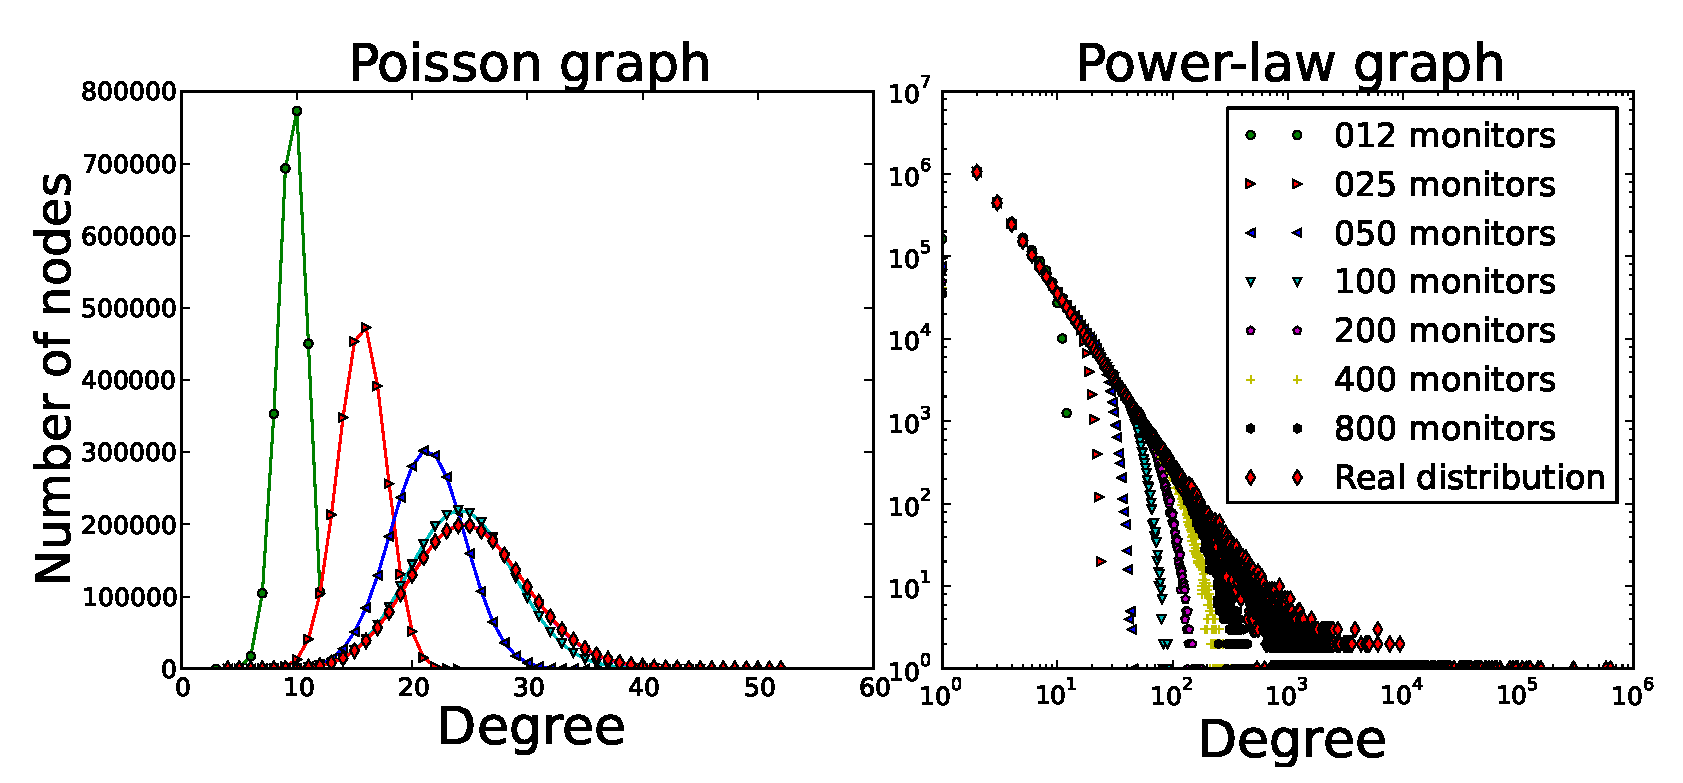
\includegraphics[width=0.49\textwidth]{figures/fig-dist-all.eps}}
\hfill
\subfigure[Scatter plot of the real degree vs. the observed degree]{\label{fig:simul.scat}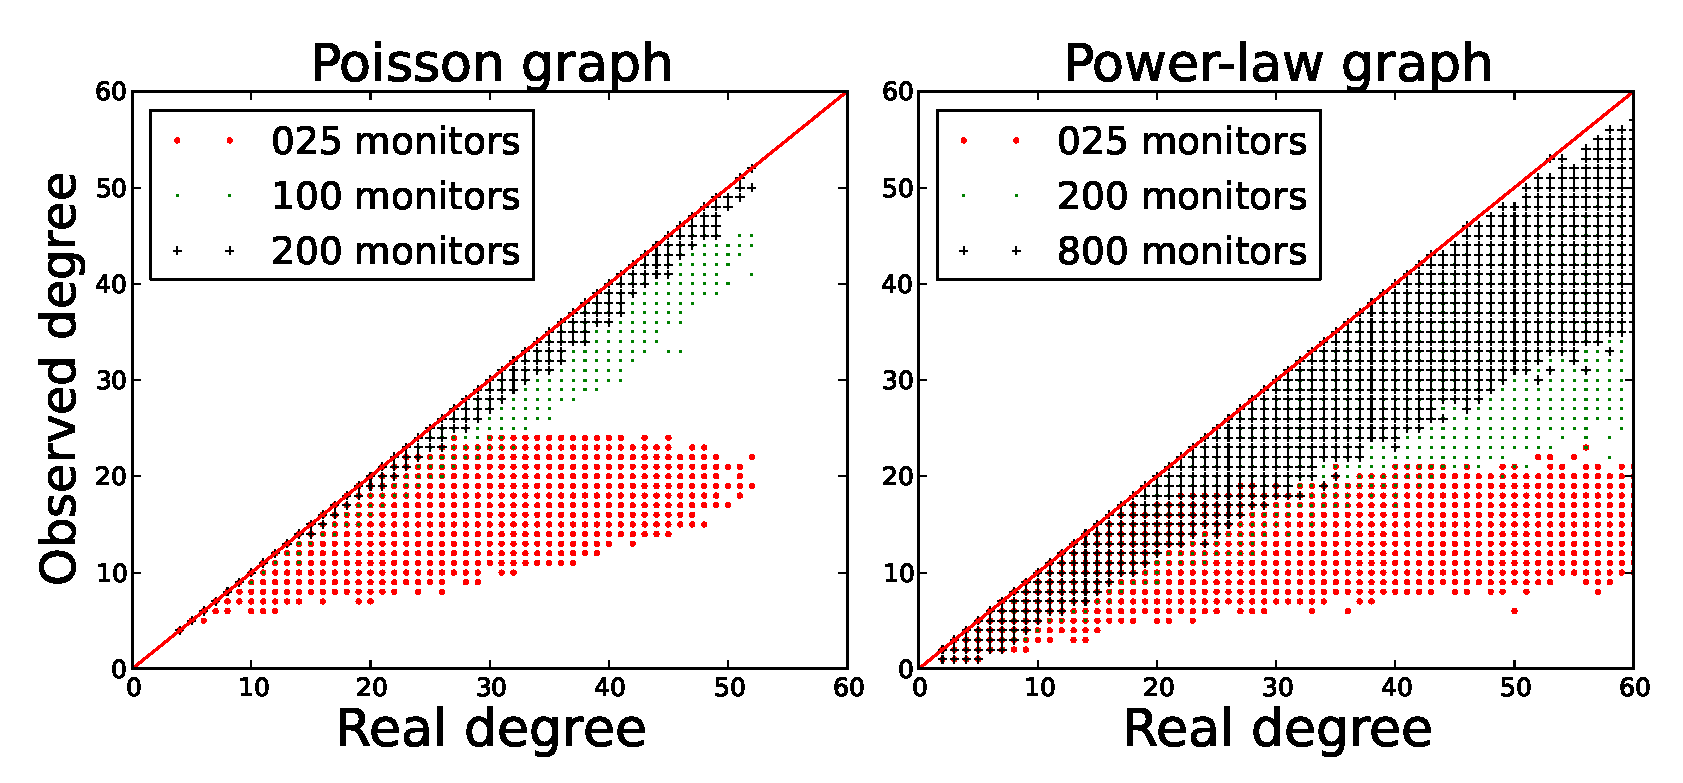
\includegraphics[width=0.49\textwidth]{figures/fig-scat-all.eps}}
\hfill
\caption{Simulations with different number of monitors (12, 25, 50, 100, 200, 400 and 800) over graphs of $2.5*10^6$ nodes whose degree distribution follows either a Poisson law with average degree $25$ or a power law with exponent $2.1$.}
\label{fig:simul}
\end{figure*}

Before putting our approach into practice, we first assess it using simulations in this section. Assuming that we are able to build appropriate sets of monitors and targets, the key questions we want to answer are: what is the risk that our estimate of a node's degree is different from its real degree, and how many monitors do we need to have an accurate estimate of the degree distribution?

To investigate this, we have conducted simulations as follows (see \cite{CT01} for more details): we considered different kinds of artificial graphs to model the topology; we used as monitors random nodes with degree one (representing end-hosts); and we used {\em all} core targets ({\em i.e.} nodes in the graph obtained by iteratively removing degree-one nodes). We then assumed that each target answers to probes from each monitor using one (randomly chosen) of its interface that starts a shortest path from the target to the monitor. We used two different kinds of topologies: one with Poisson degree distribution, which is a typical homogeneous distribution, and one with a power-law degree distribution, which is a typical heterogeneous distribution. These two kinds of distributions are considered as extreme cases for what the actual degree distribution may be.

\figurename~\ref{fig:simul} shows the results of the simulations for Poisson and power-law graphs of $2.5$ million nodes.  \figurename~\ref{fig:simul.degdist} presents the degree distribution observed with respectively 12, 25, 50, 100, 200, 400 and 800 monitors. As one could expect, with 12 monitors the degree distribution is poorly estimated in the two cases. Nevertheless, it is remarkable that, even with this poor level of quality, the nature of the distribution (\emph{i.e.} homogeneous or heterogeneous) appears clearly.  When the number of monitors increases, so does the quality of the observed degree distribution.

With $200$ monitors in particular, the observed and the real distributions become visually indistinguishable in the homogeneous case (left). For the heterogeneous case (right), one can observe a cut-off for very large degrees. As we mentioned previously, this comes from the limitation of our method we identified {\em a priori}: the observed degree cannot exceed the number of monitors, and more generally, the estimate becomes inaccurate for targets whose degree is close to the number of monitors. On the other hand, for reasonably low-degree targets, lets say up to 20, the observed distribution and the real one are visually indistinguishable with $200$ monitors.

These last statements are strengthened by the plots on \figurename~\ref{fig:simul.scat} which shows the scatter plot of real degree (on the x-axis) and observed degree (on the y-axis) for all targets and for the two kinds of topologies. We can see that with $200$ monitors, the estimate degree of all nodes is quite close to its real degree for the Poisson graphs, thus proving that our method performs very well on this kind of topology. As regards power-law graphs, we can see that using $200$ monitors, the estimate degree of low-degree nodes is quite close to the real one. More than $95\%$ of degree-2 nodes are correctly observed and this proportion drops to $85\%$ when considering all nodes whose degree is lower than $10$. This shows that, for this type of nodes at least, our method performs also very well on power-law graphs.

Therefore, the only limitation of our method in this theoretical setup seems to be the estimation of the degree of high-degree nodes in power-law graphs.  Indeed, an intrinsic limitation of our method is that we cannot obtain a degree estimate larger than the number of monitor $|M|$. However, this limitation has to be put in perspective as \figurename~\ref{fig:simul.scat} shows that, even if poorly estimated, they still cannot be confused with low-degree nodes. Whatever the number of monitors, the worst estimation (lower point on the y-axis) increases as the real degree increases. With $200$ monitors for instance, the worst estimate of a node with degree higher than $1000$ is $136$.

In conclusion, both for Poisson graphs and power-law graphs, the nature and the shape of the degree distribution are correctly observed even with a low number of monitors. In addition, the observed distribution quickly converges to the real one when the number of monitors grows. The real degree of low-degree nodes is correctly observed (also true for high-degree nodes in the homogeneous case), and a high-degree node is never observed as a low-degree node.

These remarks will turn out to be crucial in Section~\ref{sec:results}. However, the reader may wonder if these results still hold for graphs of different sizes and with different parameters, average degree for Poisson graphs and exponent for power-law graphs. These questions were investigated in \cite{CT01}, as well as the influence of some other parameters of the simulations. It turns out that the conclusions we derive here are still valid for different sizes and parameters. In particular, \cite{CT01} shows that the size of the graph has very little importance, if any, for the quality of the observation with a given number of monitors. Then, the conclusion obtained by simulations on graphs of a few millions of nodes still holds for graphs of the size of the internet.

%\noteperso{La possibilite d'observer des noeuds de degre 50 avec degre 20 est troublante...}


%%%%%%%%%%%%%%%%%%%%%%%%%%%%%%%%%%%%%%%%%%%%%%%%%%%%%%%%%%%%%%%%%%%%
%%%%%%%%%%%%%%%%%%%%%%%%%%%%%%%%%%%%%%%%%%%%%%%%%%%%%%%%%%%%%%%%%%%%
\section{Monitors} \label{sec:monitors}
%%%%%%%%%%%%%%%%%%%%%%%%%%%%%%%%%%%%%%%%%%%%%%%%%%%%%%%%%%%%%%%%%%%%
%%%%%%%%%%%%%%%%%%%%%%%%%%%%%%%%%%%%%%%%%%%%%%%%%%%%%%%%%%%%%%%%%%%%


Our method relies on the use of a large set $M$ of monitors distributed in the internet. It is crucial that this set is large enough since the accuracy of the estimation of the degrees of targets highly depends on this number (see Section~\ref{sec:concept}). On the other hand, having several monitors in the same location (typically having the same branching point) has limited interest: it is probable that most targets use the same interface to answer probes coming from these monitors (see \figurename~\ref{fig:colocated-monitors-observation}). Assessing the quality of a given set $M$ of monitors (regarding our measurement goals) is therefore crucial, and we propose here three different and complementary approaches to do so.

\begin{figure} \centering
%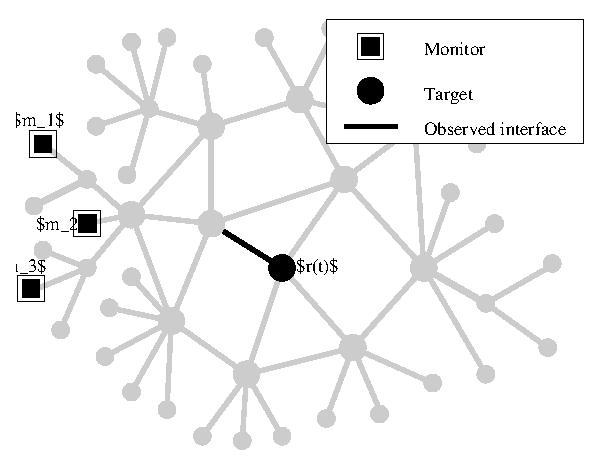
\includegraphics[width=0.95\columnwidth]{figures/colocated-monitors-observation}
\resizebox{.6\columnwidth}{!}{\input{figures/colocated-monitors-observation.pstex_t}}
\caption{Three monitors, $m_1$, $m_2$ and $m_3$ are actually colocated, and therefore they may observe a unique interface for any given target router $r(i)$. They are redundant regarding the quality of the measurement.}
\label{fig:colocated-monitors-observation}
\end{figure}

\subsection{Colocated monitors}
\label{sec:colocated}

First notice that any monitor $m$ may in principle be able to identify its branching point ({\em i.e.} the branching point between itself and core nodes, see Section~\ref{sec:approach}). Indeed, suppose that $m$ iteratively sends $k$ packets to $k$ random IP addresses (for a given integer $k$) with increasing TTLs: the first $k$ packets are sent with TTL 1, the $k$ next packets with TTL 2, and so on. Thanks to the ICMP Time-Exceeded packets issued by the nodes at distance $t$ from $m$ (we discuss below the case of machines that do not send such packets), for each value $t$ of the TTL $m$ discovers a set of interfaces at distance $t$ from $m$. We denote this set of interfaces by $i_t(m)$. Let us denote by $d(m)$ the smallest $t$ such that $|i_t(m)|>1$: $d(m)$ is the first TTL at which $m$ discovers more than just one interface. We have by definition $|i_{d(m)}(m)|>1$ and $|i_j(m)|=1$ for all $j<d(m)$. Then, the (unique) interface seen by $m$ with TTL $d(m)-1$, {\em i.e.} the unique element of $i_{d(m)}(m))$ is an interface of its branching point. See for instance the case of monitor $m_1$ in \figurename~\ref{fig:colocated-monitors-observation}, for which $d(m_1)=3$.

Now, let us consider two monitors $m$ and $m'$ such that $i_{d(m)}(m) = i_{d(m')}(m')$. In other words, the first time $m$ and $m'$ see several interfaces they see the exact same ones. Then certainly having both $m$ and $m'$ in the monitor set has little interest for our measurements: $m$ and $m'$ enter in the core internet through very close routers (probably through the same branching point, see \figurename~\ref{fig:colocated-monitors-observation})\,\footnote{Notice that this does not mean that such monitors have no interest at all and should be discarded: they may lead to observation of different interfaces of the target, in particular if it implements per-destination load-balancing~\cite{paristraceroute}.}. We say that such monitors are {\em colocated}. The number of non-colocated monitors in $M$ is a key value for estimating the quality of $M$: it basically represents the number of significantly different locations hosting monitors in $M$.

In the scheme we just described, we ignored machines that do not send ICMP Time-Exceeded packets. Because of them, we may erroneously decide that some monitors are colocated; this means that we under-estimate the quality of our monitor set, which has no important consequence in our context: the quality is only under-estimated. Similarly, it is possible that two monitors $m$ and $m'$ have different branching points but satisfy $i_{d(m)}(m) = i_{d(m')}(m')$. Again, this would make us under-estimate the quality of the monitor set and therefore we may safely ignore this. Conversely, some monitors $m$ and $m'$ may have different but similar sets $i_{d(m)}(m)$ and $i_{d(m')}(m')$, indicating that they are not colocated but located close from each other. It may be interesting to use this for a more subtle assessment of the level of distribution of monitors, but we leave this for further work.

\subsection{Diversity of views}
\label{sec:diversity-of-view}

In the approach above, we estimate an intrinsic quality of a monitor set $M$ as the number of different locations hosting a monitor. A complementary view is obtained by evaluating the quality of a measurement from $M$ towards targets in a set $T$. For instance, one may evaluate the quality of $M$ as the number of distinct interfaces observed from $M$: $Q_0(M) = \sum_{t\in T} |M(t)|$. Clearly, if $Q_0(M') > Q_0(M)$ then $M'$ may be considered as better than $M$. More subtle quality functions may be defined. In particular, it is interesting to take into account the fact that interfaces of low-degree routers are easier to observe than the ones of high-degree routers. This leads to the quality function $Q_1(M) = \sum_{t \in T} |M(t)| d(t)$ where $d(t)$ stands for the degree of target router $r(t)$. Of course we do not have the value of $d(t)$ and approximate it using the results of our measurements.

Given a quality function $Q$ like the ones above, one may assess the impact of the addition of a new monitor $m$ to the current monitor set, by calculating $Q(M)$ and $Q(M \cup \{m\})$. Ideally, one wants to maximize $Q$ to collect the most accurate set of observed interfaces while keeping $M$ as small as possible to prevent redundant measurements (which may be costly).

In practice, we will want to assess a given monitor set $M$, and to do so we will start from an empty monitor set and compute the expected quality improvement when monitors are added one by one, in a random order. The quality is expected to grow with the number of monitors, and then to reach a steady or almost steady regime meaning that adding more monitors would not improve the measurement significantly. Of course, if many monitors are colocated (for instance, if they are all at the same location), the quality will have precisely this behavior (as adding more monitors at the same location does not significantly improve the measurement). This is why this quality function approach is {\em complementary} to the colocation-based one: we will perform first the colocation and then plot the behavior of the quality function when non-colocated monitors are added, see Section~\ref{sec:results-monitors-assessment}.

\subsection{Convergence of observations}
\label{sec:convergence}

Last but not least, a clear way to assess the quality of a given monitor set regarding our measurements objectives is to directly observe how the observed fraction $p_k$ of routers of degree $k$ converges when the number of monitors grows, for all $k$. Here again, we expect these fractions to converge rapidly to a steady value, which is our final estimate. This would indicate that the last monitors we added were not necessary, and thus that we obtain an accurate view. For the same reasons as above, this is complementary to colocation analysis.


%%%%%%%%%%%%%%%%%%%%%%%%%%%%%%%%%%%%%%%%%%%%%%%%%%%%%%%%%%%%%%%%%%%%
%%%%%%%%%%%%%%%%%%%%%%%%%%%%%%%%%%%%%%%%%%%%%%%%%%%%%%%%%%%%%%%%%%%%
\section{Targets} \label{sec:targets}
%%%%%%%%%%%%%%%%%%%%%%%%%%%%%%%%%%%%%%%%%%%%%%%%%%%%%%%%%%%%%%%%%%%%
%%%%%%%%%%%%%%%%%%%%%%%%%%%%%%%%%%%%%%%%%%%%%%%%%%%%%%%%%%%%%%%%%%%%

Being able to sample a core router uniformly at random in the internet\,\footnote{{\em Uniformly at random} means that all possible elements are sampled with the same probability.} would help us much, but there is no direct way to do so. Instead, it is trivial to get IP addresses uniformly at random, as they are nothing but 32 bit integers. Of course, sampling such a random integer does not necessarily give a relevant IP address with regards to our measurement needs: it may for instance belong to an end-host or a router that does not answer our probes.  

In this section, we show how to sample uniformly at random an interface of an internet core router that correctly answers our probes, which we call a {\em correct core router}. From this sampling, which is not a {\em uniform} sampling of core routers themselves but only of the interfaces of some of them, we show in Section~\ref{sec:bias} how to estimate the degree distribution of all internet core routers.

First notice that a core router may give incorrect answers to our probes. In particular, it may give no answer at all, or it may always answer using the same interface independently of the monitor\,\footnote{Of course, more intricate behaviors are also possible, but they are very unlikely~\cite{keys2010internet} and we ignore them here.}. In these cases, our measurement procedure discovers zero or one interface for the corresponding target. Instead, if the target address belongs to a correct core router, our measurements see at least two of its interfaces (as long as monitors are reasonably well distributed). Therefore, we are able to distinguish between correct core routers and other core routers.

There is no reason to assume that the degree of core routers is correlated to whether they answer correctly to our probes or not. Indeed, low-degree core routers may {\em a priori} misbehave as well as high-degree ones, and conversely. As a consequence, the degree distribution of correct core routers is the same as the degree distribution of all core routers. We therefore focus on correct core routers here.

Let us now consider the IP address $i$ corresponding to a 32 bit integer sampled uniformly at random. If it belongs to a known class of reserved addresses~\cite{rfc1466}, if it belongs to no machine in the internet, if it belongs to a machine that does not answer to our probes, or if it belongs to an end-host, then our measurements see only one or zero interface for it: $|M(i)| \le 1$. As a consequence, we are able to distinguish between these cases and the one where $i$ belongs to a correct core router.

\begin{figure} \centering
\resizebox{.6\columnwidth}{!}{\input{figures/targets.pstex_t}}
\caption{If we target an interface $i$ that belongs to a border router $r(i)$ then our measurements may see more than one interface for $r(i)$. However, only one of them does not belong to $B(M)$, as displayed in this picture: all interfaces of $B(M)$ are marked with a small dash.
}
\label{fig:targets}
\end{figure}

If the target address $i$ belongs to a border router $r(i)$, then in most cases (see \figurename~\ref{fig:approach} (right)) our measurements see only one interface. In some cases, though, we may see more than just one interface, see \figurename~\ref{fig:targets}. Indeed, let us denote by $B(M)$ the set of all interfaces seen between monitors in $M$ and the core internet in the process described in Section~\ref{sec:colocated}: with the notations of this section, $B(M) = \cup_{m\in M}\cup_{k<d(m)} i_k(m)$. By construction, all IP addresses in $B(M)$ belong to border routers, and they are all such interfaces one may observe from monitors in $M$, see \figurename~\ref{fig:targets}. Conversely, if the target address belongs to a border router, then this router may have interfaces in $B(M)$, and these interfaces are seen from monitors in $M$. The key point here is that, our measurements see only one interface not in $B(M)$ for such routers. Therefore, we are able to distinguish them from correct core routers (for which we observe at least two interfaces not in $B(M)$).

In summary, we build target sets as follows. We sample random 32 bit integers and select the corresponding IP address $i$ if and only if probes to $i$ lead to observation of at least two interface not in $B(M)$. Such an IP address is called a {\em valid target}. It is sampled uniformly at random among interfaces of correct core internet routers.


%%%%%%%%%%%%%%%%%%%%%%%%%%%%%%%%%%%%%%%%%%%%%%%%%%%%%%%%%%%%%%%%%%%%
%%%%%%%%%%%%%%%%%%%%%%%%%%%%%%%%%%%%%%%%%%%%%%%%%%%%%%%%%%%%%%%%%%%%
\section{Bias correction} \label{sec:bias}
%%%%%%%%%%%%%%%%%%%%%%%%%%%%%%%%%%%%%%%%%%%%%%%%%%%%%%%%%%%%%%%%%%%%
%%%%%%%%%%%%%%%%%%%%%%%%%%%%%%%%%%%%%%%%%%%%%%%%%%%%%%%%%%%%%%%%%%%%

The procedure described in previous section samples uniformly at random IP addresses of interfaces of correct core routers, which we assume to be representative of all core routers. However, it does not sample uniformly at random correct core routers themselves: one has $k$ possibilities to sample a router with $k$ interfaces, so high-degree routers appear with probability higher than low-degree ones. More precisely, the probability to sample a router is proportional to its degree $k$, and so the observed fraction $p'_k$ of routers sampled with this bias having degree $k$ is proportional to $k$ times the fraction $p_k$ of routers sampled uniformly at random with degree $k$: $p'_k \sim k\cdot p_k$. As a consequence, we obtain:
$$
p_k = \frac{p'_k}{k} \cdot \frac{1}{\sum_{i>1}\frac{p'_i}{i}}
$$
where the second term is nothing but a normalization constant to ensure that $\sum_k p_k = 1$.

We may therefore use this formula to infer the true degree distribution $p_k$ from the observed one $p'_k$. However, $p'_k$ is the fraction of core routers with $k$ {\em core} interfaces: our measurements see the core interfaces of core routers, not their border interfaces (see Section~\ref{sec:approach}). We therefore have to ensure that the target generation procedure described in previous section samples {\em core} interfaces (of core routers) uniformly at random. To obtain this, we discard targets that turn out to be border interfaces. We detect them as follows: they are not observed during our measurements except if they belong to $B(M)$. In other words, a target interface $i$ of a correct core router is a border interface if and only if $i \not\in M(i)$ or $i \in B(M)$.

Finally, in addition to the sampling procedure described in Section~\ref{sec:targets}, we discard these targets. We then get from the other targets the value of $p'_k$ and infer the unbiased $p_k$ using the formula above.

Notice that the sampling bias towards high-degree routers has an important benefit. Indeed, we expect high-degree routers to be relatively rare (which will be confirmed by our measurements, see Section~\ref{sec:results}) and thus we may miss them. Uniform sampling would indeed lead to a probability $p_k$ to sample a router with degree $k$, but with our biased sampling this probability is proportional to $k\cdot p_k$, and thus higher for high-degree routers. This leads to a better estimate of $p_k$ when $k$ is large, while for small values of $k$ the quality of the estimate is ensured by the prevalence of low-degree routers.


%%%%%%%%%%%%%%%%%%%%%%%%%%%%%%%%%%%%%%%%%%%%%%%%%%%%%%%%%%%%%%%%%%%%
%%%%%%%%%%%%%%%%%%%%%%%%%%%%%%%%%%%%%%%%%%%%%%%%%%%%%%%%%%%%%%%%%%%%
\section{Measurement} \label{sec:measurement}
%%%%%%%%%%%%%%%%%%%%%%%%%%%%%%%%%%%%%%%%%%%%%%%%%%%%%%%%%%%%%%%%%%%%
%%%%%%%%%%%%%%%%%%%%%%%%%%%%%%%%%%%%%%%%%%%%%%%%%%%%%%%%%%%%%%%%%%%%
\label{sec:data-collection}
\label{sec:data-cleaning-filtering}

We present in this section a practical measurement we conducted following our approach. We describe the whole procedure step by step, as well as the obtained dataset.

We first built an initial target set by sending (from a machine in our lab) a probe to the IP addresses corresponding to 32 bit integers sampled uniformly at random. We stopped this process when we obtained correct answers ({\em i.e.} ICMP Destination Unreachable (Code 3/Port unreachable)) from 3 millions such targets (we considered that no answer would arrive after 1 minute). This took approximately 10 hours.

Our initial monitor set was composed of the approximately 700 machines of the PlanetLab platform \cite{planetlab}, which is a distributed infrastructure provided to researchers typically to conduct network measurements. Some of these potential monitors are colocated and some do not fit our requirements (they have very poor connections, for instance, or they belong to networks that filter ICMP packets). We will handle these issues below.

Given these initial target and monitor sets, we uploaded our measurement tools and the target set to each monitor and remotely asked them to send a probe to each target (in a random order to avoid situations where targets would receive many probes in a short period of time). This lasted approximately 4 hours (and so each target received at most 700 probes during this period). In order to explore the stability of our measurements, we repeated this operation three times in a row. The whole measurement (building the target set and probing each of them from each monitor three times) took less than 24 hours, with a very reasonable load for targets and monitors. At this stage, we obtained for each target its answers to the probes from all monitors (repeated three times), which we gathered onto a local machine for analysis.

Some targets and some monitors behaved incorrectly. For instance, some targets sent several answers for a unique probe. Others answered to a few monitors only, probably because of shutdowns during measurements, very low ICMP rate limiting, or other specific reasons. Conversely, some monitors received surprisingly few answers, probably due to a very poor local connections, shutdowns, or to the fact that PlanetLab machines may be overloaded (they are shared by numerous users). To avoid potential noise due to these anomalous behaviors, we first discarded targets giving multiple answers to a probe. We then observed for each monitor the number of targets that answered its probes, and conversely for each target the number of monitors that received answers from it, see \figurename~\ref{fig:filters}. These plots show that most monitors received answers from most targets, as we expected. To ensure that we only keep relevant data, we discarded monitors that received answers to less then $80\%$ of their probes, and conversely all targets that sent answers to less than $80\%$ of probes; this represents a minority of all monitors and targets, see Table~\ref{tab:summary}.

\begin{figure} \centering
\hfill \includegraphics[angle=-90,width=0.48\columnwidth]{figures/filter-monitors} \hfill \includegraphics[angle=-90,width=0.48\columnwidth]{figures/filter-targets} \hfill
\caption{Left (resp. right): for each number $x$ on the horizontal axis, we plot the number of targets (resp. monitors) that sent (resp. received) at least $x$ answers to our probes, for each of our three measurements.}
\label{fig:filters}
\end{figure}

Following the requirements of our method, we then built the set $B(M)$ of border interface seen from our monitors and we discarded all targets $t$ such that $t$ is not in the set of interfaces used bt $r(t)$ to answer probes ({\em i.e.} $t \not\in M(t)$) or $t$ is a border interface ($t \in B(M)$), see Sections~\ref{sec:targets} and~\ref{sec:bias}. Finally, we discarded all targets having only one interface not in $B(M)$ (which, as explained in Section~\ref{sec:targets}, do not belong to correct core routers).

We give the precise numbers encountered during the whole process for our three measurements in Table~\ref{tab:summary}.

\begin{table} \centering
\resizebox{.9\columnwidth}{!}{\input{table.tex}}
\smallskip
\caption{Key post-processing steps for our three measurements.}
\label{tab:summary}
\end{table}

We finally obtain for each of our three measurements approximately 5600 targets belonging to correct core routers. The key output of our measurements is the observed degree of these routers, from which we will estimate the degree distribution of internet core routers in the next section.

%\noteperso{donner le nb de routeurs de chaque degre observe ? pas la place ? pas le temps ?}

%\noteperso{Several facts are worth noticing: nb final targets, no blacklisting finally, ...}

\section{Results}
\label{sec:results}
\label{sec:observed-distrib}

The degree distributions observed from our three measurements, after bias correction following the formula of Section~\ref{sec:bias}, are given in Table~\ref{tab:distribs}. We plot the inverse cumulative distributions in \figurename~\ref{fig:distribs}.

\begin{table} \centering
\resizebox{.98\columnwidth}{!}{\input{tab_distribs_col.tex}}
\smallskip
\caption{The degree distributions obtained from our three measurements (after bias correction): for each degree $k$, we give the estimated fraction $p_k$ of core routers with degree $k$.}
\label{tab:distribs}
\end{table}

\begin{figure} \centering
\includegraphics[angle=-90,width=.9\columnwidth]{figures/final-result-icdf-loglog}
\caption{Inverse cumulative degree distribution obtained from our three measurements, after bias correction: for each value $x$ on the horizontal axis, we plot the fraction of core routers having degree higher than or equal to $x$ (log-log scale).}
\label{fig:distribs}
\end{figure}

First notice that results from each measurements are very similar, which confirms that our results are stable in this setup.

Obtained distributions show clearly that low-degree core routers are prevalent: approximately 75\% of them have degree 2 only, and almost 20\% have degree 3. This is not surprising, as we observe core interfaces only: these routers certainly have other interfaces connected to border routers and/or end-hosts. The number of interfaces they use to actually {\em route} traffic in the core internet, however, is very low.

Instead, some core routers have much larger degrees, and the highest one we observe is 29. We may possibly miss a few interfaces of this router but, as explained above, there is little chance that the true largest degree is much higher: we perform measurements from a much larger number of monitors and so the fact that observed degrees are bounded by this number plays no role. Of course, core routers with degree higher than 29 may exist, and they probably do. There is however none in our random target set and we therefore expect them to be extremely rare (which is reinforced by the sampling bias towards high-degree routers explained at the end of Section~\ref{sec:bias}).

Finally, the key point here is that the obtained degree distribution is {\em not} a power-law, as often assumed: the inverse cumulative distribution plotted in a log-log scale in \figurename~\ref{fig:distribs} would be a straight line. Instead, it is well fitted by a straight line until degree approximately $10$, but then it experiences a sharp decrease similar to an exponential cutoff and it rapidly reaches the highest degree. Fully characterizing this distribution remains to be done, but this is sufficient to conclude that the degree distribution of internet core routers is not a power-law.

\section{Assessment of results}
\label{sec:assessment}

In this section, we explore two approaches to assess the quality and robustness of our results. We first study the quality of our monitor set following the methods described in Section~\ref{sec:monitors}. We then run simulations similar to the ones in Section~\ref{sec:concept} to show that our results are self-consistent.

\subsection{Quality of the monitor set}
\label{sec:results-monitors-assessment}

%\noteperso{l'assessment devrait prendre en compte la correction du biais...}

As explained in Section~\ref{sec:colocated}, the distributed nature of our monitor set is a key feature for our measurements. We therefore ran the procedure described in this section to identify classes of colocated monitors, which provide basically redundant information. We obtained 203 different classes, each containing in average $2.11$ monitors. This is consistent with the fact that each institution involved in PlanetLab often contributes with several monitors located at the same place. Examination of the DNS names of monitors belonging to a same class confirmed this: they typically match the same *.domain.tld pattern.

Once colocated monitors are identified, we investigate the diversity of views obtained from various locations, as explained in Section~\ref{sec:diversity-of-view}: we first estimate the quality of the monitor set when only one colocation class is used, then two colocation classes, etc, until all colocation classes (and thus all monitors) are used. We add colocation classes in a random order and average the obtained quality. The result is displayed in \figurename~\ref{fig:quality-classes} (left). As expected, for both quality functions, the quality increases sharply at the beginning and rapidly converges. This indicates that adding more monitors at more locations would not improve the results much, and so that our monitor set and the number of locations hosting them are reasonable.

%\noteperso{Dans la Figure~\ref{fig:quality-classes} il faudrait enlever les valeurs des Q, qui prennent plein de place sans rien apporter, et pour l'autre sous-figure il faudrait améliorer la lisibilité}

\begin{figure} \centering
\hfill
\includegraphics[angle=-90,width=0.49\columnwidth]{figures/quality-classes}
\hfill
\includegraphics[angle=-90,width=0.49\columnwidth]{figures/classes-propdeg}
\hfill
\caption{
Left: evolution of the quality of the monitor set when we add colocation classes.
Right: convergence of the fraction of routers of degree $k$ with the number of colocation classes.
}
\label{fig:propdeg-classes}
\label{fig:quality-classes}
\end{figure}

%\begin{figure}] \centering
%  \begin{center}
%    \includegraphics[angle=-90,scale=0.33]{figures/quality-monitors}
%      \caption{Convergence of the relative quality of the monitors set with the number of monitors}
%  \end{center}
%  \label{fig:quality-monitors}
%\end{figure}

In order to deepen this, we examine the impact of adding more monitors at more locations on the observed fraction $p_k$ of core routers with degree $k$ (which is what we are interested in), as discussed in Section~\ref{sec:convergence}. We add colocation classes one by one like above and observe how $p_k$ evolves and obtain \figurename~\ref{fig:propdeg-classes}. The estimates for small degrees rapidly converges, which was expected as only few monitors (and locations) are needed to observe them. Interestingly, only very few locations (approximately 10) are needed to obtain an estimate of $p_k$ for $k<5$ with a 80\% precision. Increasing the number of monitors rapidly increases the quality of the estimate. Even for large degrees, the estimate rapidly reaches a value comparable to the final one, despite the fact that it only slowly converges after that.

Finally, this work on the monitor set shows that we have $200$ significantly different locations hosting monitors, and that this is sufficient to ensure a reasonable quality for our results. It is clear however that increasing the number of monitors and the number of locations hosting them would increase both accuracy and reliability of our estimates.

\subsection{Simulation bootstrap}

We demonstrated the relevance of our approach by simulating it on artificial graphs in Section~\ref{sec:concept}. In the lack of a better knowledge, we used two extreme degree distributions: Poisson and power-law ones. We conduct here similar simulations but with the degree distribution obtained in Section~\ref{sec:results} from our measurements. We expect our method to be able to observe this distribution accurately, otherwise the estimate we obtain above would make little sense.

We built 5~random graphs of 1 million nodes\,\footnote{Remind that the size of the graph has little impact on the obtained results, see Section~\ref{sec:concept}.} according to each of the 3~measured distributions; these graphs represent the core internet in our simulations. For each graph, we then sampled 5~different sets of nodes at random to play the role of monitors. This leads to $75$ different simulations, for which we tested sets of $12$, $25$, $50$, $100$, $200$, $400$ and $800$ monitors. As our monitors cannot be colocated in this framework (the considered graphs have no border), the simulations most similar to our PlanetLab measurements are the one with $200$ monitors.

\begin{figure} \centering
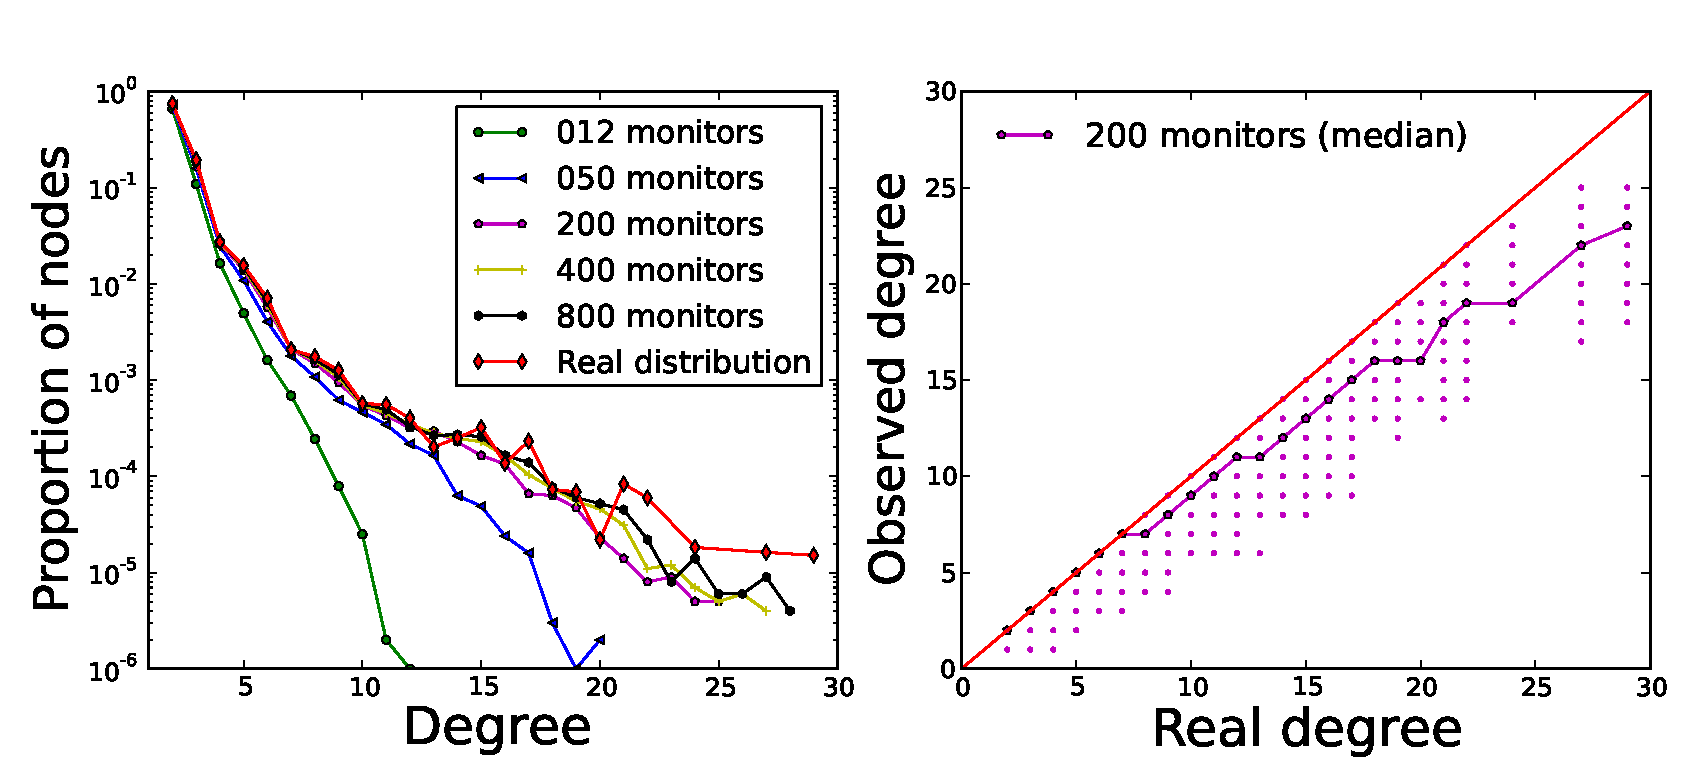
\includegraphics[width=\columnwidth]{figures/fig-valid.eps}
\caption{Assessment by simulations. Left: the observed degree distributions with various numbers of monitors. Right: correlations between observed and real degree with $200$ monitors (one dot per node and median).}
\label{fig:assess-dist}
\end{figure}

\figurename~\ref{fig:assess-dist} (left) displays the degree distributions observed with different sets of monitors. It shows that $200$ monitors in different locations is sufficient to observe the real degree distribution, even if the fraction of high-degree nodes is less accurate than others. The plot shows that the proportion of small degree nodes is particularly well approximated: $95\%$ of all nodes with degree less than or equal to $10$ are observed with their real degree with $200$ monitors.

%\noteperso{Fig~\ref{fig:assess-dist} (gauche) devrait plutot etre en log-log}

We deepen this by studying how close the observed degree of a node is to its real degree, see \figurename~\ref{fig:assess-dist} (right). This figure confirms that our method succeeds in measuring the degree of specific nodes. In particular, the median value remains close to the real one, even for the highest degrees. Moreover, even for the highest degrees, the estimated degree is never far from the real one. For instance, $18$ has been the worst estimate made for a $29$-degree node; $17$ for a $27$-degree one and $18$ for a $24$-degree one. Given the fact that these are worst cases and that we cannot over-estimate a degree, such errors remain quite low.

In conclusion, simulations of our method are in accordance with our empirical measurements: the global degree distribution (which is our focus here) observed in simulations is consistent with the real one, and the estimate of the degree of specific nodes is very accurate as long as their degree is not too high. Increasing the number of monitors would provide better estimates of the fraction of high-degree nodes, without drastically changing our conclusions.

%\noteperso{En fait ce que montrent ces simuls c'est qu'on pourrait tres bien sous-estimer les degres max, et donc peut etre avoir une power law ?? Il faudrait iterer pour voir quand ca converge...}

\section{Related work}
\label{sec:related}

The physical and IP-level internet topologies are extensively studied since the seminal papers of Pansiot {\em et al.}~\cite{280555} and Faloutsos {\em et al.}~\cite{DBLP:conf/sigcomm/FaloutsosFF99}. The most classical approach consists in building maps from traceroute-like measurements. However, several studies have shown that obtained maps are intrinsically biased~\cite{DBLP:conf/infocom/LakhinaBCX03,DBLP:journals/jacm/AchlioptasCKM09,willinger,MDBP10,DBLP:journals/tcs/DallAstaABVV06,DBLP:journals/cn/GuillaumeLM06,DBLP:conf/infocom/LatapyM08,roughan201110}, and even that traceroute outputs are unreliable~\cite{paristraceroute,pansiot2012,roughan201110}. The hope that increasing the size and quality of maps would overcome these issues has led to much effort, but the situation remains far from satisfactory~\cite{willinger,DBLP:conf/imw/BarfordBBC01,DBLP:conf/infocom/LatapyM08}.

Conducting precise measurements of the degree of random nodes to obtain a reliable estimate of the degree distribution was first suggested in~\cite{DBLP:conf/infocom/LakhinaBCX03}. We explored the possibility to do so at IP level in~\cite{CLR10} but we only partly succeeded and we conducted thorough simulations in~\cite{CT01}. Property-driven network measurement are also developed in other contexts, in particular Online Social Networks (OSNs)~\cite{kurant2011towards,gjoka2010walking} and P2P overlay measurements~\cite{stutzbach2009unbiased}.

Our work is also closely related to alias resolution (which plays a key role in the building of maps): while we seek all (unknown) interfaces of a given router identified by one of its interfaces, alias resolution aims at identifying in a given set of interfaces the ones that belong to a same router~\cite{DBLP:conf/infocom/GovindanT00,DBLP:journals/ton/GunesS09,alias-bias,keys2010internet}. Probes similar to ours are used in this context, in particular by the \emph{iffinder} tool~\cite{iffinder}, as well as other techniques. Our use of such probes was clearly inspired by these works.

Finally, important efforts are devoted to the deployment of large and distributed measurements infrastructures, which are crucial for this field of research~\cite{caida,dimes,iplane,planetlab,ripeatlas}. Some of them distribute monitoring capabilities at a huge scale (typically onto thousands of end-hosts) and so are particularly promising for us \cite{ripeatlas,dimes}.

\section{Conclusion and discussion}
\label{sec:conclusion}

In this work, we have obtained an estimate of the degree distribution of internet core routers in a rigorous way, which makes it much more reliable than previous estimates obtained from maps. To do so, we focused on the measurement of this property rather than the collection of a large (but still partial, biased and erroneous) map of the whole internet. This made it possible to design, implement and run a measurement grounded on reasonable and well identified assumptions.

Our method also has the advantage that various assessments of its results are possible. Here, in addition to the repeated measurements, we assessed the results using variations of the monitor set and simulations. Exploring other assessment approaches would increase their reliability. In particular, one may run various anti-aliasing techniques on the results of our measurements in order to confirm that the different interfaces we discover for a given target do belong to a same router. One may also run our measurements on targets for which the true degree is known, thus providing ground truth assessment.

In another direction, one may of course use larger sets of targets in order to improve the accuracy of our estimate, in particular regarding high-degree nodes. As the measurements we presented took only 4 hours, doing so seems easy. Using more and better distributed monitors would be another important improvement. In particular, most PlanteLab monitors are hosted by universities, which may induce some bias in the measurements. Up to our knowledge, the most promising infrastructures for doing so are DIMES and RIPE Atlas \cite{dimes,ripeatlas}: they already provide thousands of well distributed monitors which fit our measurement requirements. Conducting larger-scale measurements from such sets of monitors to larger sets of targets (possibly to all IPv4 address space) would lead to much more insight on the actual degree distribution of routers in the core internet.

Finally, let us notice that our measurement method is very fast and induces only a small load both on monitors and targets. This is an important feature, which makes it possible to avoid bias due to dynamics during the measurement It also opens the way to studies of the dynamics of the degree distribution at an unprecedented time scale. Going further, one may even observe the time evolution of router interfaces and use this for better modeling of the internet and its dynamics.

%We consider this work as a {\em proof of concept} for a new approach to network measurements: rather than building larger and larger (but still biased and erroneous) maps and consider their properties as estimates of the true ones, we argue that one may first identify properties of interest, then design dedicated measurement procedures able to reliably estimate them, and obtain this way accurate information on the network under concern without resorting to maps of it. We beleive that this new approach is very promising, and may increase much our knowledge of actual properties of networks, crucial for modeling and simulation purpopses. To this regard, the work presented here is a first practical application of this approach, dedicated to the degree distribution of the internet physical topology.


\medskip
\noindent
{\bf Acknowledgements.}
This work is partly supported by the European Commission EULER project (FP7 FIRE grant 258307) and by the {\em Agence Nationale de la Recherche} DynGraph grant ANR-10-JCJC-0202.

\bibliographystyle{IEEEtran}
\bibliography{IEEEabrv,biblio}


\end{document}
